\section{ER Diagrams}\label{sec:er_diagrams}

\subsection{What is an ER model?}\label{sub:what_is_an_er_model_}

An ER model is a conceptual model that can later be mapped to a logical model that describes information that will be stored in the database.

\begin{note}
    Although, we almost always use an ER diagram, it is not needed and other diagrams can be used instead.
\end{note}

\subsection{Entities}\label{sub:_entities_}

An entity represents a real world thing that we want to store data about in our database. eg. Instead of ``University of Glasgow'', we would say ``Universities''
An entity can represent a real word thing, an event, a concept, or a name (among other things).

\begin{highlight}{An entity that is used in an ER diagram}
    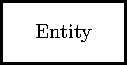
\includegraphics{lualatex/dsr/3/entity.pdf}
\end{highlight}

\subsection{Attributes}\label{sub:attributes}

An attribute is basically a property that exists on all instances of an entity.
Attributes must be kept simple, but we can have composite attributes that have many attributes of their own.

Another interesting point about attributes is that we can have multi-valued attributes which act as though they were arrays.

\begin{highlight}{An entity with attributes in an ER diagram}
    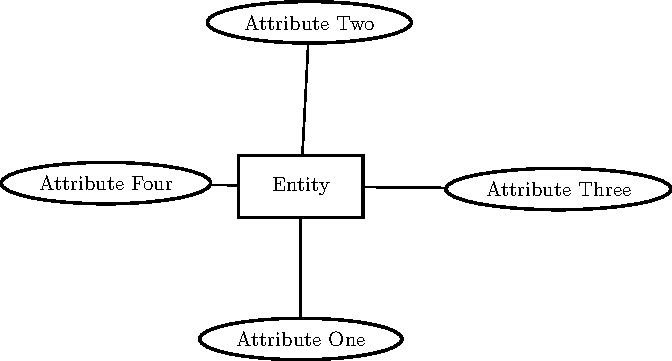
\includegraphics{lualatex/dsr/3/attribute.pdf}
\end{highlight}

\subsection{Primary Keys}\label{sub:primary_keys}

Every entity must have one or more unique attribute which we will \underline{underline}.
If there is an instance where we do no have a primary key that can be easily assigned, we can create a primary key of several keys called a \emph{compound key}.

\begin{highlight}{An entity with attributes that are primary keys in an ER diagram}
    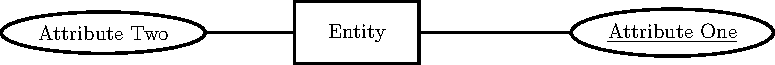
\includegraphics{lualatex/dsr/3/primarykeys.pdf}
\end{highlight}

\subsection{Subtyping}\label{sub:sub_typing}

A subtype inherits from another type (eg. A manager is an employee) just like in object oriented programming.

There are several types of subtype:
\begin{description}
    \item[Disjoint] Must belong to exactly one subtype (no more, or less), symbolised by a \(d\)
    \item[Inclusive] Can belong to any number at all, symbolised by a \(o\)
\end{description}

\begin{note}
    This is an ``is a'' relationship.
\end{note}

\begin{highlight}{An entity type with subtypes that is used in an ER diagram}
    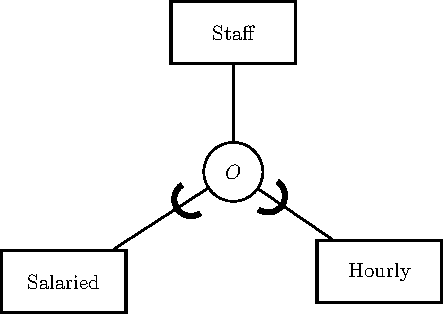
\includegraphics{lualatex/dsr/3/subtyping.pdf}
\end{highlight}

\subsection{Relationships}\label{sub:relationships}

We need to capture how \(\geq 2\) entity types are related.
We use verbs to represent the interactions between entities.

We can also have attributes on relationships, but these cannot be used to identify the relationship because one employee could come back to a department again at a later date.

There may be many relationships between the same entities (eg. ``reads report'' and ``writes report'')

An entity may also be in a relationship with itself.

\begin{highlight}{An relationship that is used in an ER diagram}
    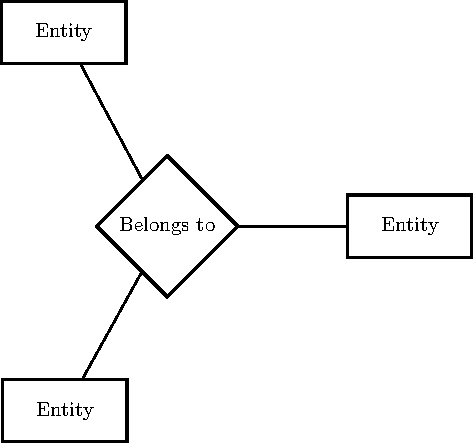
\includegraphics{lualatex/dsr/3/relationships.pdf}
\end{highlight}

\subsection{Degrees}\label{sub:degrees}

A relationship can be \emph{binary} if there are only two entities related (``an employee works in a department''), or it can be \emph{tenary} if there are more than one items (``an employee works in a department in a location'')

\begin{note}
    Non-binary relationships are \emph{very} rare in real life.
\end{note}

\subsection{Cardinality}\label{sub:cardinality}

We have different types of cardinality which represent the different relationships entities can have.
\begin{itemize}
    \item One to one (\(1:1\))
    \item One to many \(1:M\)
    \item Man to many \(M:N\)
\end{itemize}

\subsection{Participation Constraints on Relationships}\label{sub:participation_constraints_on_relationships}

A double line indicates that the relationship must contain that entity.

\begin{highlight}{A diagram showing how participation constraints are shown on an ER diagram}
    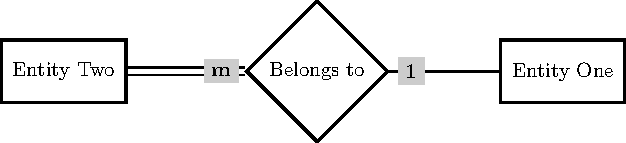
\includegraphics{lualatex/dsr/3/mandatoryrelationships.pdf}
\end{highlight}

\subsubsection{Weak Entity Types}\label{ssub:weak_entity_types}

\emph{Weak Entities} don't have primary keys of their own, so they depend on other entities to enforce uniqueness.

We don't know a unique id for our employee's children, but we do know their names, and we can assume that the names will be unique among an employee's children.

A weak entity must have complete participation in a relationship, so cannot exist by itself.

\begin{highlight}{How weak entities are represented in an ER diagram}
    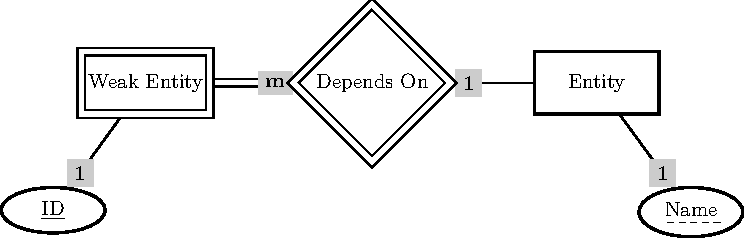
\includegraphics{lualatex/dsr/3/weakentities.pdf}
\end{highlight}

\subsection{Summary Steps}\label{sub:summary_steps}

\begin{enumerate}
    \item Create entity types
    \item Figure out properties
    \item Which ones are attributes?
    \item Which of these attributes are keys?
    \item Which of these keys are primary keys?
    \item Which properties infer relationships?
    \item Decide on the cardinality of the relationships
\end{enumerate}
